\section{Evaluation}
To evaluate the improvements and optimizations made to the JZX, we tested three versions, the original implementation, the array instruction implementation and the lazy flags implementation, to measure the time spent during the execution of an instruction. All the three implementation tested are single thread versions. To evaluate the emulator with multiple threads, we tested two versions, single thread version, and two threads version. Both versions with lazy flags. The tests consisted in playing two ZX Spectrum games,  Bombjack, 48K game, and Renegade, 128K game, for about five minutes. This tests were made in RNL's computer, with Intel Core i5 760 (Quad-core) CPU, and 8 GB of memory, running Debian 6.0 and Oracle's Java 6 JVM.

\subsection{Instruction execution}
To measure the time that each instructions takes to execute, we use the average time that two million instructions take to execute. We measure the time that every instruction takes to execute in nanoseconds and after two million instructions executed we compute the average that every instruction took to execute. With this approach we can execute and compare the performance between versions without affecting the performance of the emulator.\\
\indent In Figure 5, we present the chart that shows the evolution of the time per instruction in the Bombjack, 48K game. The value of time in original implementation, is much higher than the other versions. The time per instruction in instruction array version improved about 47\% compared to original version. Regarding the lazy flags version, we were hoping that the time per instruction had decreased, but the value of time had a slight increase of about 3\%.\\
\indent Like in Bombjack, in Renegade, a 128K game, in the original version the value of time per instruction is also higher than the improved versions. In this game, the improvement is about 43\% compared to the array instruction version. As in Bombjack, the version with lazy flags should be more efficient, but the value of time increased about 7\%.\\
\indent The lazy flags implementation goal was to make the execution of one instruction faster. But in practice, it didn't happened. This is due to a choice in our implementation. The problem lies in when we execute one instruction, instead of directly access the position in the flags array, we perform a for cycle to do that.\\
\indent As we said earlier, the goal of the implementation with threads was eliminate 30\% of the total time.\\
\indent The charts in figures x and y show that the improvement of having two threads, one processing the execution of one instruction and the other processing the update of the screen, doesn't have great impact in the total emulation time. Due to active waits the emulation time still occupies some time between execution time, making the emulation sequential.
\begin{figure}
	\center{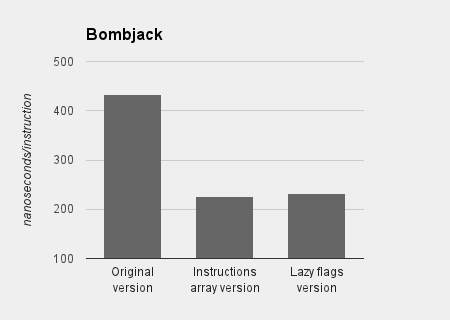
\includegraphics[width=0.4\textwidth]{img/chart_1.png}}
	\caption{Time per instruction in Bombjack}
\end{figure}
\begin{figure}
	\center{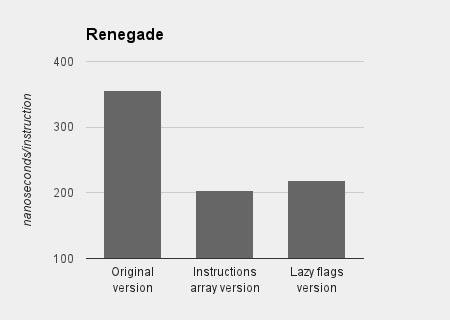
\includegraphics[width=0.4\textwidth]{img/chart_2.png}}
	\caption{Time per instruction in Renegade}
\end{figure}
\begin{figure}
	\center{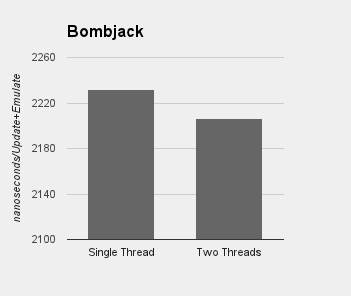
\includegraphics[width=0.4\textwidth]{img/chart_3.png}}
	\caption{Comparison time per instruction in Bombjack}
\end{figure}
\begin{figure}
	\center{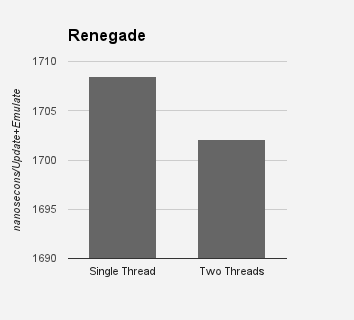
\includegraphics[width=0.4\textwidth]{img/chart_4.png}}
	\caption{Comparison time per instruction in Renegade}
\end{figure}